 \documentclass [52pt] {article}
\usepackage{amsthm}
\usepackage[margin=1in]{geometry}
\usepackage{inputenc}
\usepackage{amsmath}
\usepackage{bm}
\usepackage{afterpage}
\usepackage{hyperref}
\hypersetup{
    colorlinks=true,
    linkcolor=blue
    }
\newcommand{\norm}[1]{\left\lVert#1\right\rVert}
\newcommand{\upn}{^{(n)}}
\newcommand{\N}{\mathbb{N}}
\newcommand{\R}{\mathbb{R}}
\newcommand{\C}{\mathbb{C}}
\newcommand{\basis}{\text{span}}
\newcommand{\Hil}{\mathbf{H}}
\newcommand{\trace}{\text{trace}}
\usepackage{ams symb}
\usepackage{enumerate}
\usepackage{amsrefs}
\usepackage{graphicx}
\usepackage{listings}
%\graphicspath{{Applied Math II (Spring 2018)}}
%Here are some prob and stat commands:
\newcommand{\var}{\text{var}}
\newcommand{\cov}{\text{cov}}
\newcommand{\Exp}{\mathbb{E}}
\newcommand{\Prob}{\mathbb{P}}
\newcommand{\simind}{\overset{\text{ind}}{\sim}}
\newcommand{\simiid}{\overset{\text{iid}}{\sim}}
\DeclareMathOperator{\diag}{diag}
\title{Measuring the Effects of Starting Pitching}
\author{Lee Przybylski}


\begin{document}

\maketitle
\abstract{Betting on baseball is challenging.  One feature that makes the sport different is that moneylines usually list probable starting pitchers.  To take advantage of this, we develop a generalized linear mixed effects model using retrosheet data from several seasons.  The model includes effects for teams, starting pitchers, and venue.  Being able to assess a pitcher's performance independent of his team is also challenging.  By estimating effects for each starting pitcher, fitting the model provides another way measure a starting pitcher's effectiveness.  We also provide some background on pitching metrics that have been used in the past, such as ERA, FIP, and DRA, and compare these metrics to our estimated pitcher effects.}


\section{Introduction}

When looking to wager on the outcome of a baseball game, your sports book will usually offer three options.  You can be the runline, which places a handicap on the teams based on their estimated margin of victory.  A team with a negative runline is favored to win.  You can bet the moneyline, where there is no restrictions on the margin of victory.  Your only objective is to bet on the team that wins.  The moneyline indicates how much risk you take on.  A favored team will have a negative moneyline, and its absolute value will equal the amount needed to wager in order to win \$100.  The underdog will have a positive moneyline and equal the the amount won for a successful \$100 wager.  Finaly, you can bet the over-under, which is like a runline in that you predict the total number of runs scored in the game.
\begin{figure}[h!]
    \centering
    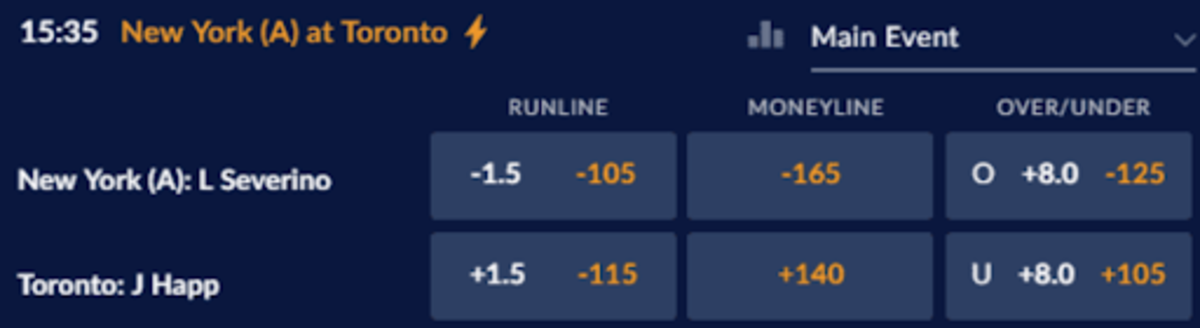
\includegraphics[scale = 0.7]{mlb-odds-2.png}
    %\caption{Caption}
    %\label{fig:my_label}
\end{figure}

We also see that the sportsbook indicates the probable starting pitchers.  We can build a regression model that will leverage the effects of starting pitchers to hopefully better predict the outcome of games.  Using the proper approach, we also can use predictors from this model to make better comparisons of starting pitchers while considering the context of who they are pitching against, where they are playing, and the quality of the defense behind them.  We will fit this model using sportsbook archive data  taken from \href{https://www.sportsbookreviewsonline.com/scoresoddsarchives/mlb/mlboddsarchives.htm}{sportsbookreviewsonline.com}.  We will compare our ratings of pitchers to other metrics such as ERA, FIP, WAR, and DRA as reported by \href{https://www.baseballprospectus.com/leaderboards/pitching/}{Baseball Prospectus}.  
\\\\
Data and code to recreate the experiments described below using R is available on Github at \href{https://github.com/przybylee/RunsScoredAnalysis}{przybylee/RunsScoredAnalysis}.

\section{Model Selection}

\subsection{Overdispersion}

When we use regression to fit a generalized linear model (GLM) with an exponential family of distributions, it is usually the case that the variance of our distribution is a function of the mean of the distribution.  Recall that a Poisson distribution with mean $\lambda>0$, denoted $\text{poiss}(\lambda)$, has pmf
\[f(x) = \frac{e^{-\lambda}\lambda^x}{x!},\:\:x\in\N_0.\]
Through a link function, we can use ordinary least squares to find an estimate for the mean based on the covariates, but often variance implied by this estimated mean is too small to explain the variation observed in the data.  When this happens, we say that the model has \emph{overdispersion}.  This must be accounted for in order to perform meaningful inference.  There are 2 common ways to deal with overdispersion.
\begin{itemize}
\item We can add a dispersion parameter to the model which is estimated using a quasi-likelihood approach.
\item We can fit a generalized linear mixed effects model (GLMEM) where we assume the mean is also affected by a centered normal random variable. 
\end{itemize}
Here we will elect to follow the second approach.

\subsection{Model Definitions}
Let $y_{ijklm}$ be the number of runs scored by team $i$ against team $j$ at venue $k$ facing starting pitcher $l$ during the $m$th game of the season.  The model we propose assumes that $y_{ijklm}\sim\text{Poisson}(\lambda_{ijklm})$ where
\begin{equation}\label{eq : model1}
\log(\lambda_{ijklm}) = \mu + \chi \mathbf{1}_{im} + b_i + f_j + v_k + p_l + g_m + e_{im},
\end{equation}
\[b_i\simiid N(0,\sigma^2_b), f_j\simiid N(0,\sigma^2_f), v_k\simiid N(0,\sigma^2_v), p_l\simiid N(0, \sigma^2_p),\:\:g_m\simiid N(0, \sigma^2_g), e_{im}\simiid N(0,\sigma^2_e).\]
\[\mathbf{1}_{im} = \begin{cases}
1 & \text{if team}\:i\:\text{is home during game}\:m\\
0 &\text{otherwise}
\end{cases}\]
We will refer to this model as the full generalized linear mixed model (FGLMM).  When fitting the FGLMM to games from the 2021 season, we find the following interesting estimates:
\begin{itemize}
    \item $\hat{\mu} = 1.36$, meaning the expected runs for the visiting team is 3.91.
    \item $\hat{\chi} = 0.036$, meaning teams tend to score 3.8\% more runs at home.
    \item $\hat{\sigma}^2_b = 0.005$ (Variance in offensive performances)
    \item $\hat{\sigma}^2_f = 0.010$ (Variance in teams overal defenses)
    \item $\hat{\sigma}^2_v = 0.007$ (Variance in park effects)
    \item $\hat{\sigma}^2_p = 0.002$ (Variance in starting pitchers)
    \item $\hat{\sigma}^2_g = 0.006$ (Variance in game effects)
    \item $\hat{\sigma}^2_e = 0.229$ (Overdispersion)
\end{itemize}
It is a bit surprising that the variance in park effects was so much larger than the variance accross starting pitchers.  This tells us that the amount of runs scored has a bigger change of change if I move the game from Guarentee Rate Field in Chicago to Coors Field in Denver, than if I change the starting pitcher from Carlos Carasco to Max Scherzer.  Intuitively, we might think the starting pitcher should matter a lot more.

\subsection{Validation Testing}

Can see by the large estimate of $\hat{\sigma}^2_e$ that there is a lot of overdispersion in our models fit.  This tells us that the FGLMM should allow for much better inference than a simpler model or a basic generalized linear model (GLM).  While convinced that the FGLMM is our better option for statistical inference, we would also like to see how well it fits the data by seeing how well it predicts the outcome of future games.  We perfom an experiment where we train the model using results from the first 15\% of the season and predict on the next 2.5\% of the season.  This is about 110 games.  We then measure measure the accuracy of our predictions, then retrain using the first 17.5\% of the season and predict on the next 2.5\% of the season.  We measure again and repeat this process for the rest of the year.

For the sake of comparison, we perform the same experiment with two other models.  The first is a simple GLM which assumes $y_{ijkl}\simiid\text{poiss}(\lambda_{ijkl})$ to be the number of runs scored by team $i$ against team $j$ at venue $k$ during game $l$, and 
\begin{equation}\label{eq : glm}
\log(\lambda_{ijkl}) = \mu + \omega_i + \delta_j + \nu_k + \chi\mathbf{1}_{ik}.
\end{equation}
The next model uses the same predictors, but treats offensive, defensive, and park effects as random.  This should give the advantage of combining information about the teams and parks to give better estimates.  This reduced GLMM assumes $y_{ijkl}\sim\text{Poisson}(\lambda_{ijklm})$ to be the number of runs scored by team $i$ against team $j$ at venue $k$, during game $l$.  We have
\begin{equation}\label{eq : glme_red}
\log(\lambda_{ijkl}) = \mu + \chi \mathbf{1}_{il} + b_i + f_j + v_k,
\end{equation}
\[b_i\simiid N(0,\sigma^2_b), f_j\simiid N(0,\sigma^2_f), v_k\simiid N(0,\sigma^2_v), p_l\simiid N(0, \sigma^2_p),\]

We perform the experiment described above for the 2021 season with all three models.  
\begin{figure}
        \centering
        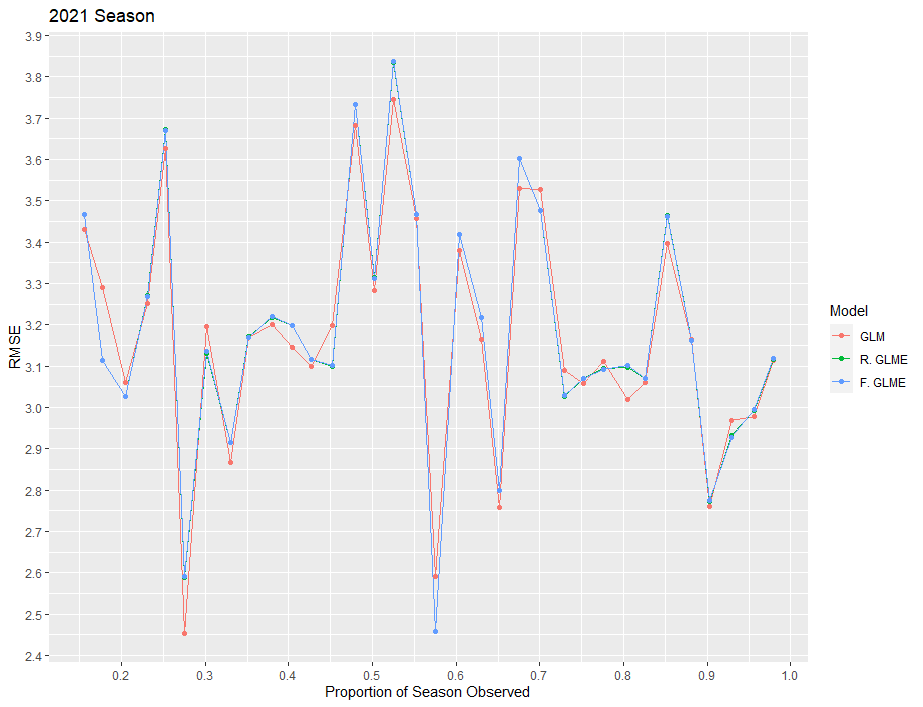
\includegraphics[scale = 0.6]{Plots/RMSE2021.png}
        \caption{Error for run predictions for validation testing during the 2021 season.  The predictions for the RGLMM follow the predictions for the FGLMM alomost perfectly.}
        \label{fig : validation_RMSE}
    \end{figure}
    
    \begin{figure}
        \centering
        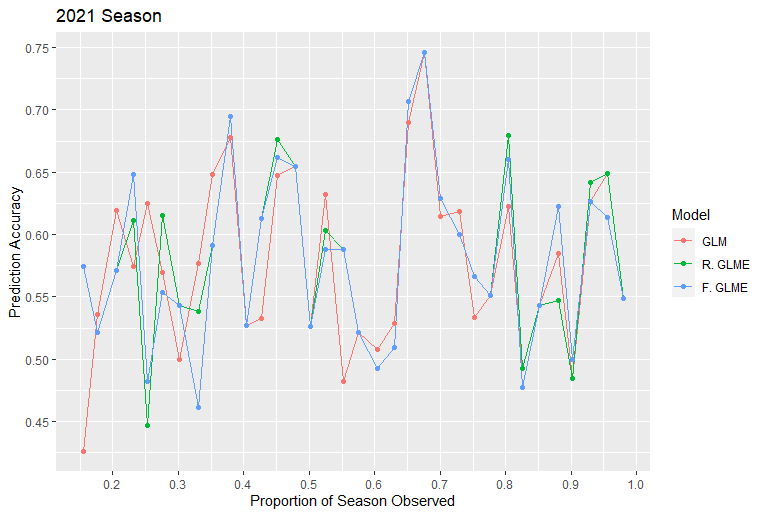
\includegraphics[scale = 0.7]{Plots/Accuracy2021.png}
        \caption{Accuracy of predictiong game outcomes during validation testing on the 2021 season.}
        \label{fig : validation_accuracy}
    \end{figure}
    
In Figure \ref{fig : validation_RMSE} we see the root-mean-squared-error (RMSE) for the predictions of the three models.  The error stays fairly close to 3.2 runs.  The RGLMM makes predictions that are fairly close to the FGLMM, so we see that the green curve is often covered by the blue curve.  It is a little surprising that the FGLMM perfromed about the same as the other two models, but it seems reasonable since there was so much variance in the overdispersion error.  We also need to note that many of the extra predictors used by the FGLMM could not be levearaged for future predictions.  There is no way to apply the best linear unbiased predictors (BLUPs) for $g_m$ and $e_{im}$ since factors depend on the particular game.  There were also games where the starting pitcher had not played yet, so we could not apply the BLUP for $p_j$ when predicting the opposing team's score.

In Figure \ref{fig : validation_accuracy} we can see that all three models could generally predict the winning team correctly about half the time.  There as a stretch when we were training with about 60\% of the season where we could predict the the winning team over 70\% of the time.  It is possible there is an optimal amount of training data.  For example, to predict on games in late September, might not requre data from March and April since these outcomes shoudl be less relevant late in the season.  The trade deadline should also be a factor.  More testing should be done to verify this theory.

\section{Pitcher Effects}

\subsection{SPR and Other Pitching Metrics}
We can extract the BLUPs for the $p_j$'s and assign a value to each pitcher.  For each pitcher, we will report $e^{\hat{p}_j}$ since this is the proportion of runs the pitcher would allow compared to the average pitcher in his environment.  We call this score the Starting Pitcher Rating (SPR).  For an example, we found that Gerit Cole had an SPR of 0.989 for the 2021 season.  This tells us that when he is starting, his team allows 1\% less runs than with the average pitcher in this situation.  A lower SPR is desired.  We can compare this metric to some of the established
pitching metrics such as ERA, FIP, and DRA, found on Baseball Prospectus.

 \begin{figure}
        \centering
        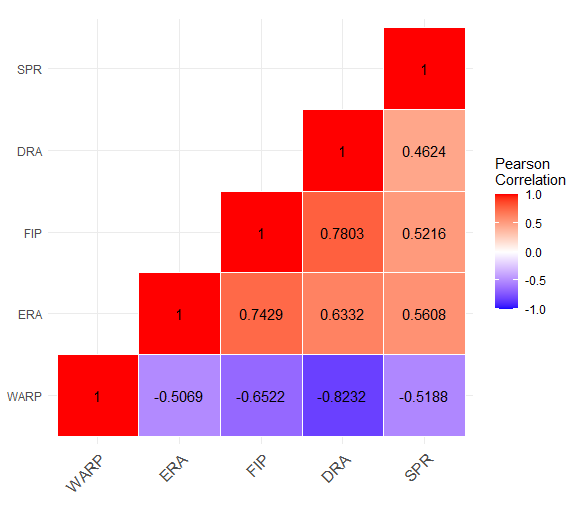
\includegraphics[scale = 0.7]{Plots/IntermetricCorr.png}
        \caption{Correlation Between Metrics in 2021}
        \label{fig : corr_metrics}
    \end{figure}
    
In Figure \ref{fig : corr_metrics}  we present the correlation coefficients for 5 metrics using starting pitchers from the 2021 season.  WARP is the Baseball Prospectus wins above replacement statistic for pitchers.  ERA is the earned run average.  FIP is fielder independent pitching, and DRA is deserved runs allowed.  Note that corrleations with WARP are negative since WARP increases with a better pitcher, while the other 4 metrics decrease.  We see in the figure that SPR correlates with WARP just as well as ERA, but is significantly behind FIP and DRA.  It is reasonable to think that SPR correlates best with ERA since these metrics are counting actual runs instead of other events that occur during the game that approximate run creation.

Another value in a pitching metric is its predictive value for future seasons.  This has been a major goal since the research by Voros McCracken in the early 2000's that lead us to FIP.  The ERA of a given pitcher has very low correlation accross different seasons.  By looking into other statistics such as BABIP, we find that this is because the pitcher has very little control of what happens once the ball is put in play.  A pitchers ERA depends on the official score keeper and his defense.  
\begin{table}[ht]
\centering
\begin{tabular}{rrrrr}
  \hline
 &2015- & 2016- & 2017- & 2018- \\ 
  \hline
\#& 140 & 138 & 151 & 163 \\ 
WARP & 0.624 & 0.560 & 0.549 & 0.474 \\ 
DRA  & 0.562 & 0.604 & 0.546 & 0.518 \\ 
FIP  & 0.421 & 0.426 & 0.353 & 0.406 \\ 
ERA & 0.226 & 0.237 & 0.228 & 0.119 \\ 
SPR & 0.158 & 0.153 & 0.103 & -0.017 \\ 
   \hline
\end{tabular}
\caption{Correlation Across Consecutive Seasons}
\label{tab : cross_ssn_corr}
\end{table}

In table \ref{tab : cross_ssn_corr}, we looked at pitching metrics for starting pitchers from seasons 2015 trhough 2018 and checked the correlation with those same statistics in the following season.  The top row, marked with a ``\#'' indicatesthe number of common starting pitchers we found accross the two seasons.  DRA seems to have the highest predictive value, but unfortunately SPR seems to have the least.  This is interesting.  Both SPR and DRA are designed by using a mixed effects model to control for the environment, but DRA is determined by specific events rather than assigning random effects for each pitcher.  It is possible that SPR would be more predictive if we only tried to predcit the run total the first 5 innings of games.  Some of the variability could be coming from who is in the bullpen to relieve these starting pitchers.


\subsection{Noteworthy Pitchers}

Although it is not yet clear what the value of SPR is, the metric does not seem to have any trouble identifying good starting pitchers.  In the following tables, we identify the top 10 pitchers from 2021 with respect to DRA, FIP, ERA, and SPR.  We provide the SPR for every pitcher in these tables.  Table \ref{tab : bottom10SPR} also shares the 10 worst pitchers we found in terms of SPR.

\begin{table}[h!]
\centering
\begin{tabular}{rllrr}
  \hline
 rank & Name & Team & DRA & SPR \\ 
  \hline
  1 & Jacob deGrom & NYM & 2.410 & 0.970 \\ 
  2 & Corbin Burnes & MIL & 2.630 & 0.963 \\ 
  3 & Taylor Rogers & MIN & 3.000 & 0.981 \\ 
  4 & Michael Kopech & CWS & 3.040 & 0.994 \\ 
  5 & Tyler Glasnow & TAM & 3.070 & 0.980 \\ 
  6 & Zack Wheeler & PHI & 3.150 & 0.961 \\ 
  7 & Brandon Woodruff & MIL & 3.180 & 0.993 \\ 
  8 & Gerrit Cole & NYY & 3.250 & 0.989 \\ 
  9 & Max Scherzer &  & 3.260 & 0.953 \\ 
 10 & Logan Webb & SFO & 3.290 & 0.973 \\ 
   \hline
\end{tabular}
\caption{Top 10 starting pitchers of 2021 according to DRA}
\label{tab : DRA}
\end{table}

\begin{table}[h!]
\centering
\begin{tabular}{rllrr}
  \hline
 rank & Name & Team & FIP & SPR \\ 
  \hline
    1 & Jacob deGrom & NYM & 1.230 & 0.970 \\ 
    2 & Corbin Burnes & MIL & 1.630 & 0.963 \\ 
    3 & Jesse Chavez & ATL & 2.010 & 0.994 \\ 
    4 & Collin McHugh & TAM & 2.120 & 0.989 \\ 
    5 & Taylor Rogers & MIN & 2.130 & 0.981 \\ 
    6 & Aaron Loup & NYM & 2.440 & 0.998 \\ 
    7 & Trevor Rogers & MIA & 2.540 & 0.981 \\ 
    8 & Tanner Houck & BOS & 2.570 & 0.996 \\ 
    9 & Zack Wheeler & PHI & 2.590 & 0.961 \\ 
   10 & Logan Webb & SFO & 2.720 & 0.973 \\ 
   \hline
\end{tabular}
\caption{Top 10 starting pitchers of 2021 according to FIP}
\end{table}

\begin{table}[h!]
\centering
\begin{tabular}{rllrr}
  \hline
  rank & Name & Team & ERA & SPR \\ 
  \hline
     1 & Aaron Loup & NYM & 0.950 & 0.998 \\ 
      2 & Jacob deGrom & NYM & 1.080 & 0.970 \\ 
      3 & Dominic Leone & SFO & 1.510 & 0.999 \\ 
     4 & Collin McHugh & TAM & 1.550 & 0.989 \\ 
      5 & Jesse Chavez & ATL & 2.140 & 0.994 \\ 
      6 & Tyler Rogers & SFO & 2.220 & 0.981 \\ 
      7 & Louis Head & TAM & 2.310 & 0.999 \\ 
      8 & Drew Smith & NYM & 2.400 & 1.008 \\ 
      9 & Corbin Burnes & MIL & 2.430 & 0.963 \\ 
     10 & Ryan Burr & CWS & 2.450 & 1.001 \\ 
   \hline
\end{tabular}
\caption{Top 10 starting pitchers of 2021 according to ERA}
\label{tab : ERA}
\end{table}

\begin{table}[ht]
\centering
\begin{tabular}{rllrrrrr}
  \hline
 rank & Name & Team & SPR & ERA & FIP & WARP & DRA \\ 
  \hline
  1 & Max Scherzer &  & 0.953 & 2.460 & 2.970 & 4.700 & 3.260 \\ 
  2 & Zack Wheeler & PHI & 0.961 & 2.780 & 2.590 & 5.800 & 3.150 \\ 
  3 & Corbin Burnes & MIL & 0.963 & 2.430 & 1.630 & 5.500 & 2.630 \\ 
  4 & Shane Bieber & CLE & 0.968 & 3.170 & 3.020 & 2.400 & 3.350 \\ 
  5 & Jacob deGrom & NYM & 0.970 & 1.080 & 1.230 & 3.300 & 2.410 \\ 
  6 & Logan Webb & SFO & 0.973 & 3.030 & 2.720 & 3.600 & 3.290 \\ 
  7 & Lance Lynn & CWS & 0.977 & 2.690 & 3.310 & 3.100 & 3.840 \\ 
  8 & Chris Flexen & SEA & 0.977 & 3.610 & 3.890 & 0.700 & 5.220 \\ 
  9 & Blake Snell & SDG & 0.978 & 4.200 & 3.820 & 2.400 & 3.930 \\ 
  10 & Robbie Ray & TOR & 0.979 & 2.840 & 3.690 & 3.900 & 3.760 \\ 
  \hline
\end{tabular}
\caption{Top 10 starting pitchers of 2021 according to SPR}
\label{tab : top10SPR}
\end{table}

\begin{table}[ht]
    \centering
    \begin{tabular}{rllrrrrr}
     \hline
 rank & Name & Team & SPR & ERA & FIP & WARP & DRA \\ 
  \hline
  218 & Carlos Carrasco & NYM & 1.020 & 6.040 & 5.220 & 0.500 & 4.770 \\ 
  219 & Aaron Nola & PHI & 1.020 & 4.630 & 3.370 & 4.300 & 3.470 \\ 
  220 & Riley Smith & ARI & 1.022 & 6.010 & 4.880 & -0.200 & 5.870 \\ 
  221 & Spenser Watkins & BAL & 1.022 & 8.070 & 6.370 & -0.900 & 6.980 \\ 
  222 & David Peterson & NYM & 1.023 & 5.540 & 4.770 & 0.600 & 4.770 \\ 
  223 & Johan Oviedo & STL & 1.023 & 4.910 & 5.270 & 0.000 & 5.560 \\ 
  224 & Jackson Kowar & KAN & 1.026 & 11.270 & 6.430 & -0.500 & 7.160 \\ 
  225 & Jake Arrieta &  & 1.030 & 7.390 & 6.170 & 0.100 & 5.460 \\ 
  226 & J.A. Happ &  & 1.032 & 5.790 & 5.130 & -1.800 & 6.600 \\ 
  227 & Dallas Keuchel & CWS & 1.036 & 5.280 & 5.220 & -2.500 & 6.890 \\ 
   \hline
\end{tabular}
\caption{Bottom 10 starting pitchers of 2021 according to SPR}
\label{tab : bottom10SPR}
\end{table}

It is a little surprising to see some big names featured on Table \ref{tab : bottom10SPR} such as Dallas Keuchel and Carlos Carrasco.  The only real surprise I found in the top 10 for SPR is Chris Flexen of Seattle.  On the otherhand, Flexen did go 14-7 this past season with the 2nd most wins in the American League.  Looking at the other names in \ref{tab : top10SPR}, it seems like having a winning record was fairly important for having a good SPR.  

\section{Conclusion}
For now we offer the following closing thoughts:

 \begin{itemize}
        \item While the model seemed to do fairly well at predicting the outcome games during the 2021 season, the problem is still challenging using only moneyline data.
        \item The SPR metric, derived from the model seemed fairly consistent with popular pitching metrics, but demonstrated little predictive value accross seasons.
        \item With the growing impact of releif pitchers, we might consider fitting a model for runs scored in the first 5 innings and derive an SPR from these blups.
    \end{itemize}

\section{Data Sources and Further Reading}
Data:\\
    \begin{itemize}
    \item\url{https://www.sportsbookreviewsonline.com/scoresoddsarchives/mlb/mlboddsarchives.htm}
    %\vspace{0.3cm}
    \item \url{https://www.baseballprospectus.com/leaderboards/pitching/}
    \end{itemize}
    \vspace{0.4cm}
    
    \noindent Further reading:
   \begin{itemize}

\item    Jonathan Judge with Baseball Prospectus on DRA:\\
    \href{https://www.baseballprospectus.com/news/article/26196/prospectus-feature-dra-an-in-depth-discussion/}{www.baseballprospectus.com/news/article/26196/prospectus-feature-dra-an-in-depth-discussion/}\\
    \vspace{0.3cm}
    
\item    Piper Slowinski with Fangraphs on FIP:\\
    \url{https://library.fangraphs.com/pitching/fip/}
    \vspace{0.3cm}
    
\item    Tom Verducci with Sports Illustrated on Starting Pitchers in 2014:\\
    \url{https://www.si.com/betting/2020/07/02/gambling-101-major-league-baseball-betting}
    
\end{itemize}


\end{document}